% AA-02 | Algebra abstrakcyjna | kanoniczny rozdzial: warstwy, izomorfizmy
% Zrodla porownawcze: TOP-02, BT-01, ALG-00. Oryginaly pozostaja niezmienione.
\chapter{Warstwy, twierdzenie Lagrange'a i grupy ilorazowe}
\label{aa:ch:lagrange-ilorazy}

\section{Warstwy: rozbijanie grupy na części tej samej wielkości}
Niech $G$ będzie grupą, a $H\le G$ jej podgrupą.
Będziemy badać, na ile elementy $G$ różnią się od siebie
z punktu widzenia $H$. Kluczowa jest obserwacja, że przesunięte
kopie $H$ są albo identyczne, albo rozłączne.

\begin{definicja}[Warstwy lewo- i prawostronne, indeks]
\label{aa:def:warstwy}
Dla $g\in G$ definiujemy \emph{warstwę lewostronną}
$gH=\{gh:h\in H\}$ oraz \emph{warstwę prawostronną}
$Hg=\{hg:h\in H\}$.
Zbiór warstw lewostronnych oznaczamy $G/H$;
na tym etapie jest to jedynie zbiór, niekoniecznie grupa.
Liczbę warstw lewostronnych nazywamy \emph{indeksem} $H$ w $G$
i zapisujemy $[G:H]$.
\end{definicja}

\begin{lemat}[Kiedy dwie warstwy są równe?]
\label{aa:lem:rowne-warstwy}
Niech $G$ będzie grupą, a $H\le G$. Dla $g_1,g_2\in G$
zachodzą równoważności
\[
 g_1H=g_2H \quad\Longleftrightarrow\quad
 g_2^{-1}g_1\in H\quad\Longleftrightarrow\quad
 g_1H\cap g_2H\ne\varnothing.
\]
Analogicznie $Hg_1=Hg_2$ dokładnie wtedy, gdy
$g_1g_2^{-1}\in H$. Każda warstwa $gH$ ma tyle elementów co $H$.
\end{lemat}
\begin{proof}
Załóżmy $g_1H=g_2H$. Ponieważ $e\in H$, mamy
$g_1=g_1e\in g_2H$, a więc $g_1=g_2h$ dla pewnego $h\in H$.
Po pomnożeniu przez $g_2^{-1}$ dostajemy $g_2^{-1}g_1=h\in H$.

Odwrotnie, jeśli $g_2^{-1}g_1=h_0\in H$, to $g_1=g_2h_0$,
a stąd $g_1H=g_2h_0H=g_2H$. Uzasadnijmy ostatnią równość:
$h_0H=H$, gdyż mnożenie z lewej przez $h_0$ ma odwrotność
mnożenia przez $h_0^{-1}$, a oba należą do $H$.

Jeśli przecięcie warstw jest niepuste, to istnieją
$h_1,h_2\in H$ z $g_1h_1=g_2h_2$.
Przekształcenie daje $g_2^{-1}g_1=h_2h_1^{-1}\in H$,
więc warstwy są równe. Równe warstwy mają oczywiście
niepuste przecięcie, ponieważ $H\ne\varnothing$.
Dla warstw prawostronnych, jeśli $Hg_1=Hg_2$, to
$g_1\in Hg_2$ i istnieje $h\in H$ takie, że $g_1=hg_2$.
Stąd $g_1g_2^{-1}=h\in H$. Odwrotnie, gdy
$g_1g_2^{-1}=h\in H$, to $Hg_1=Hhg_2=Hg_2$,
ponieważ $Hh=H$. Jeśli natomiast $Hg_1\cap Hg_2\ne\varnothing$,
to z $h_1g_1=h_2g_2$ dla pewnych $h_1,h_2\in H$
wynika $g_1g_2^{-1}=h_1^{-1}h_2\in H$;
a zatem także dwie różne warstwy prawostronne są rozłączne.

Odwzorowanie $H\to gH$, $h\mapsto gh$, jest surjekcją
z definicji warstwy, a jego różnowartościowość wynika
ze skracalności: $gh_1=gh_2$ implikuje $h_1=h_2$.
Jest więc bijekcją i $|gH|=|H|$.
\end{proof}

\begin{twierdzenie}[Rozkład na warstwy]
\label{aa:tw:podzial-warstwy}
Niech $G$ będzie grupą, a $H\le G$. Warstwy lewostronne
względem $H$ tworzą rozkład $G$ na niepuste, parami rozłączne
podzbiory. Analogiczne stwierdzenie zachodzi dla warstw prawostronnych.
Ponadto istnieje bijekcja między zbiorami warstw lewostronnych
i prawostronnych zadana przez $gH\mapsto Hg^{-1}$.
\end{twierdzenie}
\begin{proof}
Każda warstwa $gH$ zawiera $g$, bo $e\in H$, zatem jest niepusta.
Każdy $g\in G$ należy do $gH$, więc suma wszystkich warstw daje $G$.
Z lematu o równości warstw każde dwie różne warstwy są rozłączne.
Dla warstw prawostronnych mamy $g=eg\in Hg$, każda jest więc
niepusta, a ich suma wynosi $G$. Z dowodu poprzedniego lematu
dwie warstwy prawostronne są albo równe, albo rozłączne.

Sprawdźmy dobrze określoność podanej bijekcji.
Jeżeli $gH=g'H$, to $g'^{-1}g\in H$,
a po odwróceniu $g^{-1}g'\in H$.
Z kryterium warstw prawostronnych wynika
$Hg^{-1}=Hg'^{-1}$. Definiujemy więc funkcję na warstwach.
Odwzorowanie odwrotne to $Hg\mapsto g^{-1}H$;
identyczny rachunek pokazuje, że jest dobrze określone.
Obie kompozycje są identycznościami, gdyż $(g^{-1})^{-1}=g$.
\end{proof}

\begin{przyklad}[Warstwy w $\mathbb Z$]
W grupie addytywnej $G=\mathbb Z$ i dla $H=4\mathbb Z$
warstwy to $0+H$, $1+H$, $2+H$, $3+H$.
Na przykład $1+H=\{\ldots,-7,-3,1,5,9,\ldots\}$.
Zupełny podział na cztery warstwy to po prostu podział liczb
całkowitych według reszty z dzielenia przez $4$.
Ponieważ dodawanie jest przemienne, warstwy lewo- i prawostronne
nie różnią się od siebie.
\end{przyklad}

\begin{przyklad}[Warstwy w grupie nieabelowej]
\label{aa:prz:warstwy-s3}
W $S_3$ niech $H=\{e,(1\,2)\}$. Mamy trzy warstwy lewostronne:
\[
 H,\quad (1\,3)H=\{(1\,3),(1\,2\,3)\},\quad
 (2\,3)H=\{(2\,3),(1\,3\,2)\}.
\]
Wystarczy wykonać składanie zgodnie z konwencją od prawej do lewej.
Przykładowo $(1\,3)(1\,2)=(1\,2\,3)$.
Natomiast $H(1\,3)=\{(1\,3),(1\,3\,2)\}$,
więc $(1\,3)H\ne H(1\,3)$.
Warstwy istnieją bez normalności podgrupy, ale nie muszą być
takie same po lewej i po prawej stronie.
\end{przyklad}

\begin{figure}[htbp]
\centering
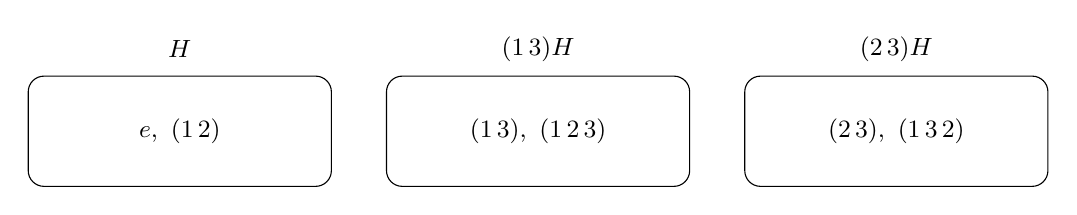
\begin{tikzpicture}[font=\small,
  every node/.style={align=center},
  box/.style={draw,rounded corners=2mm,minimum height=1.40cm,minimum width=3.85cm}]
  \node[box] at (0,0) {$e,\ (1\,2)$};
  \node at (0,1.04) {$H$};
  \node[box] at (4.55,0) {$(1\,3),\ (1\,2\,3)$};
  \node at (4.55,1.04) {$(1\,3)H$};
  \node[box] at (9.10,0) {$(2\,3),\ (1\,3\,2)$};
  \node at (9.10,1.04) {$(2\,3)H$};
\end{tikzpicture}
\caption{Rozkład $S_3$ na trzy rozłączne warstwy lewostronne względem
$H=\{e,(1\,2)\}$. Każda warstwa ma dwa elementy.}
\label{aa:fig:warstwy-s3}
\end{figure}

\section{Twierdzenie Lagrange'a i jego konsekwencje}
\begin{twierdzenie}[Lagrange'a]
\label{aa:tw:lagrange}
Niech $G$ będzie grupą skończoną, a $H\le G$. Wtedy
$|G|=[G:H]\,|H|$. W szczególności $|H|$ dzieli $|G|$.
\end{twierdzenie}
\begin{proof}
Z twierdzenia o rozkładzie $G$ na warstwy każda warstwa
lewostronna jest niepusta, a dwie różne warstwy są rozłączne.
Z lematu o warstwach każda z nich ma dokładnie $|H|$ elementów.
Ponieważ $G$ jest skończona, jest tylko skończenie wiele warstw;
oznaczmy ich liczbę przez $k=[G:H]$.
Możemy wypisać $G=g_1H\,\dot\cup\,\cdots\,\dot\cup\,g_kH$,
gdzie symbol $\dot\cup$ oznacza sumę rozłączną.
Licząc elementy sumy rozłącznej otrzymujemy
$|G|=\sum_{i=1}^{k}|g_iH|=\sum_{i=1}^{k}|H|=k|H|$.
Jest to dokładnie żądany wzór. Ponieważ $k$ jest dodatnią
liczbą całkowitą, $|H|$ dzieli $|G|$.
\end{proof}

\begin{wniosek}[Rząd elementu dzieli rząd grupy]
\label{aa:wn:rzad-dzieli}
Niech $G$ będzie grupą skończoną. Dla każdego $g\in G$
liczba $\operatorname{ord}(g)$ dzieli $|G|$, a ponadto $g^{|G|}=e$.
\end{wniosek}
\begin{proof}
Podgrupa $\langle g\rangle\le G$ ma z definicji
$\operatorname{ord}(g)$ elementów. Twierdzenie Lagrange'a
zastosowane do tej podgrupy daje
$\operatorname{ord}(g)\mid |G|$.
Zapiszmy $|G|=k\operatorname{ord}(g)$.
Z definicji rzędu i twierdzenia o grupach cyklicznych
$g^{\operatorname{ord}(g)}=e$, zatem
$g^{|G|}=(g^{\operatorname{ord}(g)})^k=e$.
\end{proof}

\begin{wniosek}[Grupa rzędu będącego liczbą pierwszą]
\label{aa:wn:p-cykliczna}
Niech $p$ będzie liczbą pierwszą, a $G$ grupą rzędu $p$.
Wówczas $G$ jest cykliczna.
W szczególności jest abelowa.
\end{wniosek}
\begin{proof}
Ponieważ $p>1$, istnieje $g\in G$ z $g\ne e$.
Podgrupa $\langle g\rangle$ ma co najmniej dwa elementy,
więc jej rząd jest dzielnikiem $p$ większym od $1$.
Jedynym takim dzielnikiem liczby pierwszej jest $p$.
Zatem $|\langle g\rangle|=|G|$ i $\langle g\rangle=G$.
Grupa cykliczna jest abelowa na mocy twierdzenia z rozdziału poprzedniego.
\end{proof}

\begin{przyklad}[Co wynika z rzędu, a co nie wynika?]
Twierdzenie Lagrange'a podaje warunek konieczny, ale nie
zapewnia istnienia elementu każdego rzędu będącego dzielnikiem
rzędu grupy. Na przykład w grupie $A_4$ rzędu $12$
nie ma elementu rzędu $6$, choć $6\mid12$.
Rzeczywiście elementy $A_4$ to tożsamość, osiem $3$-cykli
oraz trzy iloczyny dwóch rozłącznych transpozycji.
Ich rzędy to odpowiednio $1$, $3$ i $2$.
Zatem żaden z nich nie ma rzędu $6$.
Nie utożsamiamy też istnienia elementu rzędu $d$ z istnieniem
podgrupy rzędu $d$: kierunek od elementu do podgrupy zachodzi
przez $\langle g\rangle$, lecz odwrotnie podgrupa może nie być cykliczna.
\end{przyklad}

\begin{wniosek}[Grupa rzędu $2p$ dla $p$ pierwszego: obserwacja]
Niech $p$ będzie liczbą pierwszą, a $G$ grupą rzędu $2p$.
Wtedy każdy element $G$ ma rząd należący do
$\{1,2,p,2p\}$, z pominięciem powtórzeń, jeśli $p=2$.
Jest to tylko ograniczenie arytmetyczne: nie oznacza,
że elementy wszystkich wymienionych rzędów muszą istnieć,
i nie klasyfikuje struktury grupy.
\end{wniosek}
\begin{proof}
Dzielnikami $2p$ są wymienione liczby, a z poprzedniego wniosku
rząd każdego elementu musi być jednym z nich.
\end{proof}

\section{Grupa jednostek modulo \texorpdfstring{$n$}{n} i twierdzenie Eulera}
Przy obliczaniu odwrotności modulo $n$ wykorzystamy tożsamość
Bézouta, którą udowodniliśmy w Lemacie~\ref{aa:lem:bezout}.
Pokazuje ona, że dla $\gcd(a,n)=1$ istnieją
$u,v\in\mathbb Z$ z $ua+vn=1$.


\begin{definicja}[Jednostki modulo $n$]
\label{aa:def:jednostki}
Dla liczby całkowitej $n\ge2$ definiujemy
\[
 (\mathbb Z/n\mathbb Z)^\times
 =\{[a]_n\in\mathbb Z/n\mathbb Z:\gcd(a,n)=1\}.
\]
Działaniem jest mnożenie klas modulo $n$. Liczbę tych klas
oznaczamy $\varphi(n)$ i nazywamy \emph{funkcją Eulera}.
\end{definicja}

\begin{lemat}[Dlaczego jednostki są grupą?]
\label{aa:lem:jednostki-grupa}
Dla każdej liczby całkowitej $n\ge2$ zbiór $(\mathbb Z/n\mathbb Z)^\times$
stanowi skończoną grupę abelową o rzędzie $\varphi(n)$.
\end{lemat}
\begin{proof}
Zapis $[a]_n$ zależy tylko od reszty z dzielenia przez $n$.
Jeżeli $a\equiv b\pmod n$, to $\gcd(a,n)=\gcd(b,n)$,
ponieważ wspólne dzielniki $a,n$ są tymi samymi liczbami,
które dzielą $b=a+kn$ i $n$.
Warunek wzajemnej pierwszości jest więc dobrze określony dla klas.

Jeśli $\gcd(a,n)=\gcd(b,n)=1$, to $\gcd(ab,n)=1$.
Wykażmy to bez nieudowodnionego jeszcze lematu Euklidesa.
Z tożsamości Bézouta wybierzmy $u,v,u',v'\in\mathbb Z$ takie,
że $ua+vn=1$ i $u'b+v'n=1$. Mnożąc równości,
otrzymujemy
\[
1=uu'ab+n(uav'+vu'b+vv'n).
\]
Każdy wspólny dzielnik $ab$ i $n$ dzieli prawą stronę
tej równości, a więc dzieli $1$. Stąd $\gcd(ab,n)=1$
i iloczyn dwóch jednostek ponownie jest jednostką.
Klasa $[1]_n$ jest neutralna i należy do tego zbioru.

Z tożsamości Bézouta istnieją liczby całkowite $u,v$ z
$ua+vn=1$. Redukując modulo $n$, otrzymujemy
$[u]_n[a]_n=[1]_n$. Ponadto $\gcd(u,n)=1$:
każdy wspólny dzielnik $u$ i $n$ dzieliłby $ua+vn=1$.
Zatem $[u]_n$ także należy do zbioru jednostek i jest
odwrotnością $[a]_n$. Łączność i przemienność dziedziczą się
z mnożenia liczb całkowitych. Rząd grupy jest z definicji równy
liczbie klas o reprezentancie względnie pierwszym z $n$,
czyli $\varphi(n)$.
\end{proof}

\begin{twierdzenie}[Eulera]
\label{aa:tw:euler}
Niech $n\in\mathbb Z$, $n\ge2$, oraz $a\in\mathbb Z$ spełniają
$\gcd(a,n)=1$. Wtedy $a^{\varphi(n)}\equiv1\pmod n$.
\end{twierdzenie}
\begin{proof}
Z poprzedniego lematu klasa $[a]_n$ jest elementem
skończonej grupy $(\mathbb Z/n\mathbb Z)^\times$,
której rząd wynosi $\varphi(n)$. Z wniosku z twierdzenia
Lagrange'a dla dowolnego elementu grupy $U$ rzędu $|U|$
mamy $u^{|U|}=e_U$. Tutaj $e_U=[1]_n$,
zatem $[a]_n^{\varphi(n)}=[1]_n$.
Z definicji mnożenia klas lewa strona to
$[a^{\varphi(n)}]_n$, a równość klas jest równoważna
kongruencji zapisanej w tezie.
\end{proof}

\begin{twierdzenie}[Małe twierdzenie Fermata]
\label{aa:tw:fermat}
Jeżeli $p$ jest liczbą pierwszą i $a\in\mathbb Z$,
to $a^p\equiv a\pmod p$. Jeśli dodatkowo $p\nmid a$,
to $a^{p-1}\equiv1\pmod p$.
\end{twierdzenie}
\begin{proof}
Gdy $p\nmid a$, każda z klas $[1]_p,\ldots,[p-1]_p$
jest odwracalna: dla $1\le k<p$ mamy $\gcd(k,p)=1$.
Stąd $\varphi(p)=p-1$, więc twierdzenie Eulera daje
$a^{p-1}\equiv1\pmod p$. Po pomnożeniu przez $a$
otrzymujemy $a^p\equiv a\pmod p$.
Jeżeli $p\mid a$, to $a\equiv0\pmod p$, a więc zarówno
$a^p$, jak i $a$ mają resztę zero; pierwszy wzór zachodzi również wtedy.
\end{proof}

\begin{twierdzenie}[Wzór na funkcję Eulera]
\label{aa:tw:phi-wzor}
Niech $n\ge2$ będzie liczbą całkowitą, a
$p_1,\ldots,p_r$ wszystkimi różnymi dzielnikami pierwszymi $n$.
Wtedy
$\varphi(n)=n\prod_{i=1}^{r}(1-1/p_i)$.
W szczególności $\varphi(p^k)=p^k-p^{k-1}$
dla każdej liczby pierwszej $p$ i $k\in\mathbb N$, $k\ge1$.
\end{twierdzenie}
\begin{proof}
Wśród $n$ kolejnych liczb $1,2,\ldots,n$ dokładnie
$n/p_i$ jest podzielnych przez $p_i$; to wielokrotności
$p_i,2p_i,\ldots,(n/p_i)p_i$.
Liczba jest względnie pierwsza z $n$ dokładnie wtedy,
gdy nie jest podzielna przez żaden z $p_i$.
Z zasady włączeń i wyłączeń liczba takich liczb wynosi
\[
 n-\sum_i\frac n{p_i}+\sum_{i<j}\frac n{p_ip_j}
 -\cdots+(-1)^r\frac n{p_1\cdots p_r}.
\]
Każdy iloczyn wybranych spośród różnych liczb pierwszych
$p_1,\ldots,p_r$ dzieli $n$. Stąd wszystkie składniki
w powyższym rachunku są całkowitymi liczbami zliczanych wielokrotności. Rozwinięcie iloczynu
$\prod_i(1-1/p_i)$ daje dokładnie powyższą sumę podzieloną
przez $n$. Dla potęgi $p^k$ występuje tylko jeden
różny czynnik pierwszy, więc
$\varphi(p^k)=p^k(1-1/p)=p^k-p^{k-1}$.
\end{proof}

\begin{przyklad}[Liczenie dużych potęg modulo $15$]
\label{aa:prz:euler15}
Ponieważ $15=3\cdot5$, mamy
$\varphi(15)=15(1-1/3)(1-1/5)=8$.
Liczby względnie pierwsze z $15$ w zakresie od $1$ do $15$
to $1,2,4,7,8,11,13,14$, więc grupę jednostek można też
bezpośrednio wypisać. Twierdzenie Eulera mówi, że
$2^8\equiv1\pmod{15}$. Stąd
$2^{100}=2^{8\cdot12+4}\equiv(2^8)^{12}2^4
\equiv16\equiv1\pmod{15}$.
Zauważmy, że jest to poprawna redukcja potęgi $2$
ze względu na $\gcd(2,15)=1$.
Przy $a=3$ tego twierdzenia użyć nie wolno:
$3^8\equiv6\pmod{15}$, a nie $1$.
\end{przyklad}

\begin{przyklad}[Odwrotność z tożsamości Bézouta]
W grupie $(\mathbb Z/26\mathbb Z)^\times$ klasa $[7]$
jest odwracalna, bo $\gcd(7,26)=1$.
Algorytm Euklidesa daje $26=3\cdot7+5$,
$7=1\cdot5+2$, $5=2\cdot2+1$, a więc
$1=5-2\cdot2=3\cdot5-2\cdot7=3\cdot26-11\cdot7$.
Zatem $[7]^{-1}=[-11]=[15]$ modulo $26$;
sprawdzenie: $7\cdot15=105\equiv1\pmod{26}$.
\end{przyklad}

\begin{uwaga}[Kongruencja Fermata nie jest testem rozstrzygającym pierwszość]
Dla liczby całkowitej $m\ge2$ kongruencja
$a^{m-1}\equiv1\pmod m$ nie oznacza, że $m$ jest liczbą pierwszą.
Na przykład $341=11\cdot31$
jest złożona, ale $2^{10}=1024=3\cdot341+1$,
więc $2^{340}=(2^{10})^{34}\equiv1\pmod{341}$.
Jest to przykład liczby pseudopierwszej przy podstawie $2$.
Sam test jednej podstawy nie dowodzi pierwszości liczby.
\end{uwaga}

\section{Homomorfizmy, jądra i obrazy}
\begin{definicja}[Homomorfizm grup]
\label{aa:def:hom}
Niech $(G,\cdot)$ i $(K,\star)$ będą grupami.
Funkcję $f:G\to K$ nazywamy \emph{homomorfizmem}, jeśli
$f(xy)=f(x)\star f(y)$ dla wszystkich $x,y\in G$.
Jeżeli jest przy tym różnowartościowa, nazywamy ją
\emph{monomorfizmem}; jeśli jest surjektywna ---
\emph{epimorfizmem w sensie surjektywnego homomorfizmu grup};
a jeśli jest bijektywna --- \emph{izomorfizmem}.
Izomorfizm $G\to G$ to \emph{automorfizm} grupy $G$.
Przy istnieniu izomorfizmu $G\to K$ piszemy $G\cong K$.
\emph{Jądro} i \emph{obraz} homomorfizmu to odpowiednio
$\ker f=\{g\in G:f(g)=e_K\}$ oraz
$\operatorname{im}f=\{f(g):g\in G\}$.
\end{definicja}

\begin{lemat}[Działanie homomorfizmu na element neutralny i odwrotności]
\label{aa:lem:hom-podstawy}
Dla homomorfizmu $f:G\to K$ mamy $f(e_G)=e_K$,
$f(g^{-1})=f(g)^{-1}$ i $f(g^m)=f(g)^m$
dla wszystkich $g\in G$ i $m\in\mathbb Z$.
\end{lemat}
\begin{proof}
Z tożsamości $e_Ge_G=e_G$ wynika
$f(e_G)f(e_G)=f(e_G)$. Mnożąc przez odwrotność
$f(e_G)$, otrzymujemy $f(e_G)=e_K$.
Ponieważ $gg^{-1}=g^{-1}g=e_G$,
$ f(g)f(g^{-1})=f(g^{-1})f(g)=e_K$;
jednoznaczność odwrotności daje drugi wzór.
Dla $m=0$ trzeci wzór ma postać $f(e_G)=e_K$.
Jeżeli $f(g^m)=f(g)^m$ dla $m\ge0$, to
$f(g^{m+1})=f(g^m)f(g)=f(g)^{m+1}$.
Wreszcie dla $m=-k<0$, $k\ge1$, mamy
$f(g^m)=f((g^{-1})^k)=f(g^{-1})^k=(f(g)^{-1})^k=f(g)^m$.
\end{proof}

\begin{twierdzenie}[Jądro i obraz]
\label{aa:tw:jadro-obraz}
Dla każdego homomorfizmu grup $f:G\to K$ jądro jest
podgrupą $G$, a obraz podgrupą $K$. Homomorfizm $f$
jest różnowartościowy dokładnie wtedy, gdy $\ker f=\{e_G\}$.
Ponadto dla wszystkich $g\in G$ i $x\in\ker f$
zachodzi $gxg^{-1}\in\ker f$.
\end{twierdzenie}
\begin{proof}
Mamy $f(e_G)=e_K$, więc jądro nie jest puste.
Jeśli $x,y\in\ker f$, to
$f(xy^{-1})=f(x)f(y)^{-1}=e_Ke_K=e_K$,
zatem $xy^{-1}\in\ker f$. Z kryterium podgrupy jądro jest podgrupą.
Podobnie obraz zawiera $e_K$, a dla
$u=f(x)$ i $v=f(y)$ mamy $uv^{-1}=f(xy^{-1})$
należące do obrazu.

Jeżeli $f$ jest różnowartościowy i $f(x)=e_K=f(e_G)$,
to $x=e_G$, więc jądro jest trywialne.
Jeżeli jądro jest trywialne i $f(x)=f(y)$,
to $f(y^{-1}x)=e_K$; zatem $y^{-1}x=e_G$ i $x=y$.
Wreszcie $f(gxg^{-1})=f(g)e_Kf(g)^{-1}=e_K$.
\end{proof}

\begin{przyklad}[Homomorfizm wyznacznika]
Dla każdego ciała $K$ i $n\ge1$ wzór
$\det:\operatorname{GL}_n(K)\to K^\times$
jest homomorfizmem, gdyż $\det(AB)=\det A\det B$.
Jego jądrem jest $\operatorname{SL}_n(K)$.
Jego obraz to całe $K^\times$: liczba $a\ne0$
jest wyznacznikiem macierzy diagonalnej
$\operatorname{diag}(a,1,\ldots,1)$.
Nie jest to homomorfizm addytywny macierzy;
strukturą grupową po obu stronach jest mnożenie.
\end{przyklad}

\section{Podgrupy normalne i konstrukcja grupy ilorazowej}
\begin{definicja}[Podgrupa normalna]
\label{aa:def:normalna}
Niech $G$ będzie grupą, a $N\le G$. Podgrupę $N$
nazywamy \emph{normalną}, zapis $N\trianglelefteq G$,
jeżeli $gNg^{-1}=N$ dla każdego $g\in G$.
\end{definicja}

\begin{twierdzenie}[Równoważne kryteria normalności]
\label{aa:tw:normalna-warstwy}
Niech $G$ będzie grupą, a $N\le G$.
Następujące warunki są równoważne:
\begin{enumerate}
\item $N\trianglelefteq G$;
\item $gN=Ng$ dla każdego $g\in G$;
\item $gng^{-1}\in N$ dla wszystkich $g\in G$ i $n\in N$.
\end{enumerate}
\end{twierdzenie}
\begin{proof}
Równość $gNg^{-1}=N$ po przemnożeniu obu stron z prawej
przez $g$ daje $gN=Ng$, a odwrotnie pomnożenie przez $g^{-1}$
daje (1). Stąd (1) i (2) są równoważne.
(1) implikuje (3) przez definicję. Jeśli zachodzi (3),
to $gNg^{-1}\subseteq N$; stosując (3) do $g^{-1}$,
otrzymujemy $g^{-1}Ng\subseteq N$. Po sprzężeniu przez $g$
wyprowadzamy $N\subseteq gNg^{-1}$, co daje równość (1).
\end{proof}

\begin{twierdzenie}[Iloraz grupy przez podgrupę normalną]
\label{aa:tw:iloraz}
Niech $G$ będzie grupą, a $N\trianglelefteq G$.
Na zbiorze warstw $G/N$ wzór
$(gN)(hN)=(gh)N$ jest dobrze określony i czyni $G/N$
grupą. Element neutralny to $N=eN$,
a odwrotnością $gN$ jest $g^{-1}N$.
Odwzorowanie $q:G\to G/N$, $q(g)=gN$, jest surjektywnym
homomorfizmem, a jego jądro to $N$.
Jeżeli zaś dla dowolnej podgrupy $H\le G$ wzór
$(gH)(hH)=ghH$ jest dobrze określony na warstwach,
to $H$ musi być normalna.
\end{twierdzenie}
\begin{proof}
Załóżmy najpierw normalność $N$.
Niech $gN=g'N$ i $hN=h'N$.
Z lematu o warstwach istnieją $n_1,n_2\in N$ takie,
że $g'=gn_1$ i $h'=hn_2$. Wówczas
$g'h'=gn_1hn_2=gh(h^{-1}n_1h)n_2$.
Ponieważ $N$ jest normalna, mamy $h^{-1}n_1h\in N$;
ponieważ jest podgrupą, iloczyn $(h^{-1}n_1h)n_2$ też należy do $N$.
Otrzymujemy zatem $g'h'N=ghN$.
Wynik nie zależy od wybranych reprezentantów.

Łączność działania warstw wynika z łączności w $G$:
$((gN)(hN))(kN)=((gh)k)N=(g(hk))N=(gN)((hN)(kN))$.
Mamy $(eN)(gN)=gN=(gN)(eN)$ oraz
$(gN)(g^{-1}N)=eN=(g^{-1}N)(gN)$.
Zatem $G/N$ jest grupą.

Równość $q(gh)=ghN=(gN)(hN)=q(g)q(h)$
dowodzi, że $q$ jest homomorfizmem. Każda warstwa
jest postaci $q(g)$, więc jest on surjektywny.
Ponadto $q(g)=N$ dokładnie wtedy, gdy $g\in N$,
zatem $\ker q=N$.

Na koniec niech wzór działa dla pewnej podgrupy $H$.
Dla każdego $g\in G$, $h\in H$ mamy $hH=H$,
więc z poprawności iloczynu
$(gH)(hH)(g^{-1}H)=(gH)(H)(g^{-1}H)=H$.
Ale lewa strona według wzoru to $(ghg^{-1})H$.
Stąd $ghg^{-1}\in H$. Ponieważ dotyczy to każdego $g,h$,
uzyskujemy normalność $H$ z poprzedniego twierdzenia.
\end{proof}

\begin{wniosek}[Podgrupy normalne jako jądra]
\label{aa:wn:normalna-jadro}
Niech $G$ będzie grupą, a $N\le G$. Wówczas $N\trianglelefteq G$
dokładnie wtedy, gdy istnieje grupa $K$ i homomorfizm
$f:G\to K$, dla którego $N=\ker f$.
\end{wniosek}
\begin{proof}
Jeżeli $N$ jest normalna, twierdzenie o grupie ilorazowej
konstruuje homomorfizm $q:G\to G/N$ z jądrem $N$.
Jeżeli natomiast $N=\ker f$, to dla każdego $g\in G$
i $n\in N$ zachodzi
$f(gng^{-1})=f(g)f(n)f(g)^{-1}=e_K$,
zatem $gng^{-1}\in N$. Kryterium normalności dowodzi tezy.
\end{proof}

\begin{przyklad}[Dlaczego naturalny iloczyn warstw może nie istnieć]
Niech $H=\{e,(1\,2)\}\le S_3$.
Mamy $(1\,3)(1\,2)(1\,3)=(2\,3)\notin H$,
więc $H$ nie jest normalna.
Pokażmy zależność od reprezentantów bezpośrednim rachunkiem.
Niech $g=(1\,3)$, $g'=(1\,2\,3)$ i $k=(1\,3)$.
Ponieważ $g'=g(1\,2)$, mamy $gH=g'H$. Jeśli jednak
zastosujemy proponowany wzór do tych samych dwóch warstw,
wybierając jako reprezentanta pierwszej odpowiednio $g$ albo $g'$,
otrzymamy
\[
(gk)H=eH=H,\qquad (g'k)H=(2\,3)H\ne H.
\]
Ostatnia nierówność wynika z $(2\,3)\notin H$.
Zatem ten sam iloczyn warstw miałby dwie różne wartości:
normalność jest warunkiem koniecznym jego dobrej określoności.
\end{przyklad}

\begin{przyklad}[Iloraz $S_3/A_3$]
Niech $A_3=\{e,(1\,2\,3),(1\,3\,2)\}$.
Jest to podgrupa rzędu $3$; składa się z permutacji parzystych.
Znak permutacji $\operatorname{sgn}:S_3\to\{\pm1\}$
jest homomorfizmem (znak iloczynu to iloczyn znaków),
a jego jądrem jest $A_3$. Wynika stąd normalność $A_3$.
Z twierdzenia Lagrange'a indeks $[S_3:A_3]=6/3=2$,
więc iloraz ma dwie klasy. Funkcja
$gA_3\mapsto\operatorname{sgn}(g)$ jest dobrze określona:
przedstawiciele tej samej warstwy różnią się o element jądra
znaku. Jest bijektywna i zachowuje mnożenie, a więc
$S_3/A_3\cong\{\pm1\}\cong\mathbb Z/2\mathbb Z$.
Warto podkreślić, że warstwa nie jest pojedynczą permutacją:
jedna zawiera trzy permutacje parzyste, druga trzy nieparzyste.
\end{przyklad}

\begin{wniosek}[Podgrupy indeksu dwa są normalne]
\label{aa:wn:indeks-dwa}
Niech $G$ będzie grupą, a $H\le G$ podgrupą o indeksie $2$.
Wtedy $H\trianglelefteq G$.
\end{wniosek}
\begin{proof}
Istnieją dokładnie dwie warstwy lewostronne:
$H$ oraz $G\setminus H$, bo warstwy rozkładają $G$
i jedna z nich jest równa $H$.
Z bijekcji warstw lewo- i prawostronnych otrzymanej wcześniej
wynika, że istnieją dokładnie dwie warstwy prawostronne:
$H$ oraz $G\setminus H$.
Dla $g\in H$ mamy $gH=H=Hg$.
Dla $g\notin H$ warstwa $gH$ jest różna od $H$,
więc musi być równa $G\setminus H$; tak samo $Hg$.
Zatem $gH=Hg$ dla wszystkich $g$,
co jest równoważne normalności.
\end{proof}

\begin{przyklad}[Dlaczego $A_4$ nie ma podgrupy rzędu $6$?]
\label{aa:prz:a4-bez-szostki}
Przypomnijmy, że $A_4$ składa się z dwunastu permutacji
parzystych czterech elementów: identyczności, ośmiu $3$-cykli
i trzech produktów dwóch rozłącznych transpozycji.
Załóżmy, że $H\le A_4$ ma rząd $6$.
Wtedy $[A_4:H]=2$, więc na mocy poprzedniego wniosku
$H\trianglelefteq A_4$ i iloraz $A_4/H$ jest grupą rzędu $2$.
Każdy $3$-cykl $c$ spełnia $c^3=e$, a jego klasa
$cH$ spełnia $(cH)^3=H$.
Z twierdzenia Lagrange'a rząd $cH$ dzieli $2$;
jednocześnie z $(cH)^3=H$ wynika, że dzieli także $3$.
Jedynym wspólnym dodatnim dzielnikiem $2$ i $3$ jest $1$,
więc $cH=H$, czyli $c\in H$.
W ten sposób $H$ zawierałaby wszystkie osiem $3$-cykli
oraz element neutralny, czyli co najmniej dziewięć elementów.
To sprzeczne z $|H|=6$. Zatem taka podgrupa nie istnieje.
Ten przykład pokazuje, że odwrotność twierdzenia Lagrange'a
jest fałszywa nawet dla stosunkowo małych grup.
\end{przyklad}

\section{Twierdzenia o izomorfizmie i odpowiedniości}
\begin{twierdzenie}[Pierwsze twierdzenie o izomorfizmie grup]
\label{aa:tw:izo-pierwsze}
Jeżeli $f:G\to K$ jest homomorfizmem grup, to istnieje
dokładnie jeden izomorfizm
$\overline f:G/\ker f\to\operatorname{im}f$
spełniający $\overline f(g\ker f)=f(g)$ dla każdego $g\in G$.
\end{twierdzenie}
\begin{proof}
Niech $N=\ker f$. Z twierdzenia o jądrach wynika normalność $N$,
a więc $G/N$ jest grupą.
Aby sprawdzić, że zadany wzór określa funkcję,
załóżmy $gN=hN$. Z lematu o warstwach $h^{-1}g\in N$,
więc $f(h)^{-1}f(g)=f(h^{-1}g)=e_K$ i $f(g)=f(h)$.
Wartość wzoru nie zależy zatem od reprezentanta klasy.

Jest to homomorfizm, bo
$\overline f((gN)(hN))=f(gh)=f(g)f(h)
=\overline f(gN)\overline f(hN)$.
Jest surjektywny na $\operatorname{im}f$ z definicji obrazu.
Jeśli $\overline f(gN)=e_K$, to $f(g)=e_K$, a więc
$g\in N$ i $gN=N$; jądro $\overline f$ jest trywialne.
Z kryterium iniektywności jest więc izomorfizmem.
Wreszcie każda klasa ma postać $gN$, toteż wymagany
wzór wyznacza $\overline f$ jednoznacznie.
\end{proof}

\begin{przyklad}[Od dzielenia z resztą do izomorfizmu]
Homomorfizm grup addytywnych $f:\mathbb Z\to\mathbb Z/12\mathbb Z$
ma postać $f(k)=[k]_{12}$. Jego jądro to $12\mathbb Z$,
a obraz to cała $\mathbb Z/12\mathbb Z$. Pierwsze twierdzenie
o izomorfizmie daje $\mathbb Z/12\mathbb Z\cong\operatorname{im}f$.
Ten przykład może wydawać się tautologiczny, ale pokazuje schemat:
grupę ilorazową uzyskujemy przez utożsamienie elementów,
których obrazy pod homomorfizmem są takie same.
\end{przyklad}

\begin{twierdzenie}[Drugie twierdzenie o izomorfizmie]
\label{aa:tw:izo-drugie}
Niech $G$ będzie grupą, $H\le G$, $N\trianglelefteq G$.
Wtedy $HN=\{hn:h\in H,n\in N\}$ jest podgrupą $G$,
$N\trianglelefteq HN$, $H\cap N\trianglelefteq H$ i istnieje
naturalny izomorfizm $H/(H\cap N)\cong HN/N$.
\end{twierdzenie}
\begin{proof}
Zbiór $HN$ zawiera $e=ee$. Niech $h_1n_1,h_2n_2\in HN$.
Mamy
$(h_1n_1)(h_2n_2)^{-1}
=h_1n_1n_2^{-1}h_2^{-1}
=(h_1h_2^{-1})(h_2n_1n_2^{-1}h_2^{-1})$.
Pierwszy czynnik należy do $H$, drugi do $N$ dzięki normalności.
Stąd wynik należy do $HN$ i kryterium podgrupy daje $HN\le G$.
Normalność $N$ w $HN$ wynika z normalności w $G$.

Rozważmy homomorfizm $f:H\to HN/N$,
$f(h)=hN$. Mnożenie warstw jest dobrze określone,
ponieważ $N\trianglelefteq HN$. Każdy element $HN/N$
ma postać $hnN=hN$, więc $f$ jest surjektywny.
Jądro to $\{h\in H:hN=N\}=H\cap N$.
Pierwsze twierdzenie o izomorfizmie daje
$H/(H\cap N)\cong HN/N$. Ponieważ $H\cap N$ jest
jądrem homomorfizmu $f$, jest normalna w $H$.
\end{proof}

\begin{twierdzenie}[Trzecie twierdzenie o izomorfizmie]
\label{aa:tw:izo-trzecie}
Niech $G$ będzie grupą, $N\trianglelefteq G$ i $M\trianglelefteq G$,
przy $N\subseteq M$. Wtedy $M/N\trianglelefteq G/N$ oraz
$(G/N)/(M/N)\cong G/M$.
\end{twierdzenie}
\begin{proof}
Zdefiniujmy $F:G/N\to G/M$ wzorem $F(gN)=gM$.
Jeżeli $gN=hN$, to $h^{-1}g\in N\subseteq M$,
więc $gM=hM$; wzór jest dobrze określony.
Ponadto $F((gN)(hN))=ghM=(gM)(hM)$,
zatem $F$ jest homomorfizmem.
Jest surjektywny, ponieważ każda klasa $gM$ ma
przeciwobraz $gN$. Jego jądro składa się z tych $gN$,
dla których $gM=M$, czyli $g\in M$.
Zatem $\ker F=M/N$. Jako jądro jest to normalna podgrupa $G/N$.
Pierwsze twierdzenie o izomorfizmie, zastosowane do $F$,
daje dokładnie żądany izomorfizm.
\end{proof}

\begin{twierdzenie}[Odpowiedniość podgrup]
\label{aa:tw:odpowiedniosc}
Niech $G$ będzie grupą, $N\trianglelefteq G$ i niech $q:G\to G/N$
będzie homomorfizmem ilorazowym. Odwzorowania
$H\mapsto H/N$ oraz $K\mapsto q^{-1}(K)$ są wzajemnie
odwrotnymi bijekcjami między podgrupami $H\le G$
zawierającymi $N$ a podgrupami $K\le G/N$.
Odpowiedniość zachowuje inkluzję, a $H$ jest normalna w $G$
dokładnie wtedy, gdy $H/N$ jest normalna w $G/N$.
\end{twierdzenie}
\begin{proof}
Niech $H$ będzie podgrupą $G$ zawierającą $N$.
Wtedy $N\trianglelefteq H$, więc $H/N$ jest podgrupą $G/N$.
Przeciwobraz podgrupy przez homomorfizm jest podgrupą:
rzeczywiście zawiera element neutralny i jest zamknięty
na $xy^{-1}$, ponieważ $q(xy^{-1})=q(x)q(y)^{-1}$.
Zatem oba przyporządkowania mają wskazane przeciwdziedziny.

Dla $H$ zachodzi $q^{-1}(H/N)=H$.
Dla każdego $h\in H$ klasa $q(h)=hN$ należy do $H/N$,
co daje inkluzję $H\subseteq q^{-1}(H/N)$.
Jeżeli $g\in q^{-1}(H/N)$, to $gN=hN$ dla pewnego $h\in H$,
a więc $h^{-1}g\in N\subseteq H$.
Ponieważ $h\in H$, otrzymujemy $g\in H$.

Dla podgrupy $K\le G/N$ mamy
$q(q^{-1}(K))=K$, bo $q$ jest surjektywny.
Ta równość oznacza dokładnie $(q^{-1}(K))/N=K$.
Oba przyporządkowania są więc wzajemnie odwrotne.
Oczywiście zachowują inkluzję, ponieważ zarówno obraz,
jak i przeciwobraz zachowują inkluzje odpowiednich zbiorów.

Jeśli $H\trianglelefteq G$, to dla $g\in G,h\in H$
mamy $(gN)(hN)(gN)^{-1}=(ghg^{-1})N\in H/N$,
więc $H/N\trianglelefteq G/N$.
W drugą stronę, gdy $H/N$ jest normalna, to
$(ghg^{-1})N\in H/N$, a z równości przeciwobrazu
$q^{-1}(H/N)=H$ wynika $ghg^{-1}\in H$.
Zatem $H\trianglelefteq G$.
\end{proof}

\begin{przyklad}[Podgrupy $\mathbb Z/12\mathbb Z$ z odpowiedniości]
Podgrupy $\mathbb Z$ zawierające $12\mathbb Z$ są dokładnie
$d\mathbb Z$ dla $d\mid12$:
z klasyfikacji podgrup $\mathbb Z$ wiemy, że są to
$\mathbb Z,2\mathbb Z,3\mathbb Z,4\mathbb Z,6\mathbb Z,12\mathbb Z$.
Po przejściu do ilorazu otrzymujemy sześć podgrup
$\mathbb Z/12\mathbb Z$. Jest to druga droga do listy
podgrup otrzymanej przy badaniu grup cyklicznych.
\end{przyklad}

\section{Sprzężenia, komutatory i abelianizacja}
\begin{definicja}[Sprzężenie, centrum, komutator]
Niech $G$ będzie grupą. Dla $g,x\in G$ element $gxg^{-1}$
nazywamy \emph{sprzężonym} do $x$. \emph{Centrum} grupy to
$Z(G)=\{z\in G:zx=xz\text{ dla każdego }x\in G\}$.
\emph{Komutatorem} elementów $x,y$ nazywamy
$[x,y]=xyx^{-1}y^{-1}$.
\emph{Podgrupa pochodna} lub \emph{komutatorowa}
$[G,G]$ to podgrupa generowana przez wszystkie komutatory
$[x,y]$ dla $x,y\in G$.
\end{definicja}

\begin{lemat}[Własności centrum i podgrupy komutatorowej]
\label{aa:lem:komutatory}
Dla każdej grupy $G$ zbiory $Z(G)$ i $[G,G]$ są normalnymi
podgrupami $G$. Ponadto $G/[G,G]$ jest abelowa i jeśli
$N\trianglelefteq G$ oraz $G/N$ jest abelowa, to $[G,G]\subseteq N$.
\end{lemat}
\begin{proof}
Centrum zawiera $e$. Jeśli $z,w\in Z(G)$ i $x\in G$,
to z równości $wx=xw$ po pomnożeniu z lewej i z prawej
przez $w^{-1}$ dostajemy $w^{-1}x=xw^{-1}$. Wobec tego
$(zw^{-1})x=z(w^{-1}x)=z(xw^{-1})=(xz)w^{-1}
=x(zw^{-1})$, więc centrum jest podgrupą.
Dla $z\in Z(G)$ i $g\in G$ mamy $gzg^{-1}=z$,
więc centrum jest normalne.

Dla dowolnego $g\in G$ sprzężenie komutatora jest komutatorem:
$g[x,y]g^{-1}=[gxg^{-1},gyg^{-1}]$.
Zatem sprzężenie przez $g$ zachowuje zbiór generatorów
$[G,G]$ i jego podgrupę; stosując także $g^{-1}$,
otrzymujemy równość sprzężonej podgrupy z $[G,G]$.

W ilorazie przez $[G,G]$ zachodzi dla dowolnych $x,y\in G$
\[
 (x[G,G])(y[G,G])(x[G,G])^{-1}(y[G,G])^{-1}
 =[x,y][G,G]=[G,G].
\]
To znaczy, że dowolne dwie klasy komutują.
Odwrotnie, jeśli $G/N$ jest abelowa, to
$[xN,yN]=N$ i stąd $[x,y]\in N$ dla wszystkich $x,y$.
Ponieważ $N$ jest podgrupą zawierającą wszystkie komutatory,
zawiera też podgrupę przez nie generowaną.
\end{proof}

\begin{definicja}[Abelianizacja]
\label{aa:def:abelianizacja}
Grupę abelową $G^{\mathrm{ab}}=G/[G,G]$ nazywamy
\emph{abelianizacją} grupy $G$.
\end{definicja}

\begin{twierdzenie}[Własność uniwersalna abelianizacji]
\label{aa:tw:abelianizacja}
Niech $G$ będzie grupą, a $A$ grupą abelową.
Każdy homomorfizm $f:G\to A$ ma dokładnie jedno
faktoryzowanie przez rzut $q:G\to G^{\mathrm{ab}}$,
tzn. istnieje dokładnie jeden homomorfizm
$\overline f:G^{\mathrm{ab}}\to A$ taki, że $f=\overline f\circ q$.
\end{twierdzenie}
\begin{proof}
Dla dowolnych $x,y\in G$ w grupie abelowej $A$ mamy
$f([x,y])=f(x)f(y)f(x)^{-1}f(y)^{-1}=e_A$.
Zatem wszystkie komutatory należą do $\ker f$.
Ponieważ jądro jest podgrupą, $[G,G]\subseteq\ker f$.
Możemy więc zdefiniować
$\overline f(g[G,G])=f(g)$.
Jeżeli $g[G,G]=h[G,G]$, to $h^{-1}g\in[G,G]\subseteq\ker f$,
więc $f(g)=f(h)$. Wzór nie zależy od reprezentanta.
Dla dowolnych $g,h\in G$ zachodzi
$\overline f((g[G,G])(h[G,G]))=f(gh)=f(g)f(h)$,
czyli $\overline f$ zachowuje mnożenie.
Równość $f=\overline f\circ q$
zachodzi dla każdego $g$ z konstrukcji.
Jednoznaczność wynika z surjektywności $q$: homomorfizm
$\overline f$ musi mieć wartość $f(g)$ na każdej klasie $q(g)$.
\end{proof}

\begin{przyklad}[Abelianizacja $S_3$]
\label{aa:prz:ab-s3}
Homomorfizm znaku $\operatorname{sgn}:S_3\to\{\pm1\}$
ma jądro $A_3$, więc iloraz $S_3/A_3$ jest abelowy.
Z lematu o komutatorach wynika $[S_3,S_3]\subseteq A_3$.
Z drugiej strony dla $x=(1\,2)$, $y=(2\,3)$ mamy
$[x,y]=xyxy=(xy)^2=(1\,3\,2)$,
ponieważ $x^2=y^2=e$ i $xy=(1\,2\,3)$.
Ten komutator generuje całe $A_3$, więc
$A_3\subseteq[S_3,S_3]$. Otrzymujemy
$[S_3,S_3]=A_3$ i $S_3^{\mathrm{ab}}\cong\mathbb Z/2\mathbb Z$.
\end{przyklad}

\section{Twierdzenie Cayleya i zamknięcie pierwszego etapu}
\begin{twierdzenie}[Cayleya]
\label{aa:tw:cayley}
Każda grupa $G$ jest izomorficzna z podgrupą grupy
$\operatorname{Sym}(G)$ wszystkich permutacji swojego zbioru elementów.
Jeżeli $|G|=n<\infty$, jest więc izomorficzna z podgrupą $S_n$.
\end{twierdzenie}
\begin{proof}
Dla każdego $g\in G$ zdefiniujmy funkcję
$L_g:G\to G$ przez $L_g(x)=gx$.
Jest bijekcją: $L_{g^{-1}}(L_g(x))=g^{-1}(gx)=x$
i $L_g(L_{g^{-1}}(x))=g(g^{-1}x)=x$.
Zatem $L_g\in\operatorname{Sym}(G)$.
Zdefiniujmy $\Lambda:G\to\operatorname{Sym}(G)$,
$\Lambda(g)=L_g$. Dla $g,h,x\in G$ mamy
$(L_g\circ L_h)(x)=g(hx)=(gh)x=L_{gh}(x)$.
Zatem $\Lambda(gh)=\Lambda(g)\Lambda(h)$:
$\Lambda$ jest homomorfizmem.

Aby wykazać różnowartościowość, nie trzeba porównywać
wszystkich wartości funkcji: jeśli $L_g=L_h$, to ich
wartości w $e$ są równe, czyli $g=L_g(e)=L_h(e)=h$.
Obraz $\Lambda(G)$ jest podgrupą $\operatorname{Sym}(G)$,
a $\Lambda:G\to\Lambda(G)$ jest izomorfizmem.
Dla $n$-elementowego $G$ wybierzmy bijekcję
$b:G\to\{1,\ldots,n\}$. Przyporządkowanie
$\sigma\mapsto b\circ\sigma\circ b^{-1}$
jest izomorfizmem $\operatorname{Sym}(G)\to S_n$,
a więc obraz $\Lambda(G)$ odpowiada podgrupie $S_n$.
\end{proof}

\begin{przyklad}[Regularna reprezentacja $\mathbb Z/3\mathbb Z$]
Niech $G=(\mathbb Z/3\mathbb Z,+)$, z elementami $[0],[1],[2]$.
Translacja $L_{[1]}$ daje cykl
$[0]\mapsto[1]\mapsto[2]\mapsto[0]$,
a więc po ponumerowaniu elementów jest $3$-cyklem.
Translacja $L_{[2]}=L_{[1]}^2$ jest cyklem przeciwnym,
a $L_{[0]}$ identycznością. W ten sposób
$G$ reprezentuje się jako trójelementowa podgrupa $S_3$.
Twierdzenie nie mówi, że $G=S_3$; mówi o podgrupie
izomorficznej z $G$.
\end{przyklad}

\begin{uwaga}[Co dalej?]
W kolejnym rozdziale działania grup, orbity i stabilizatory
dostarczą silniejszego języka do liczenia elementów i analizowania
sprzężeń; wyprowadzimy też równanie klas. W następnym rozdziale
przejdziemy do twierdzenia Cauchy'ego i twierdzeń Sylowa.
Zapis iloczynu tensorowego $A\otimes_{\mathbb Z}B$
dla \emph{grup abelowych} $A,B$ wprowadzimy w rozdziale o modułach.
Jest to iloczyn tensorowy $\mathbb Z$-modułów; dla ogólnych
nieabelowych grup standardowy iloczyn tensorowy modułów nie jest
tą samą konstrukcją i wymagałby innej definicji.
\end{uwaga}
